BitBucket and GitHub offer a bunch of browser-based tools supporting code review and comments. 
Jonathan now prefers this method of providing feedback rather than writing comments in files.
One merit is that the history of feedback persists without cluttering up active code.
Another is that threaded conversations are much cleaner than writing back-and-forth within code.

Note: BitBucket offers some experimental features from time to time, 
which might change the interface and make the following instructions not applicable. 
Please opt out experimental features by going to ``Settings - Labs", 
and disable all the ``BETA" features.

\subsection{Default code review process}\label{code_review_process}
Given a task, the default process for writing code and submitting it for review is the following:
\begin{enumerate}
\item Create a new branch when you create a new task (\href{https://github.com/gslab-econ/ra-manual/wiki/Tasks}{G\&S}: ``The assignee should create a separate git branch for each task that involves code or output stored in the repository.'')
\item Commit your work on this new branch. A complete task includes a \texttt{Makefile}.
\item In addition to creating a \texttt{code} folder, write a \texttt{readme.md} in the task folder that explains what it does.
\item Submit a pull request when your code is ready to be reviewed.
\item Team uses the pull request to review code and have a conversation about the task
\item Additional commits are made on the branch in response to discussion and feedback.
\item Finalized task is added to master branch using \href{https://bitbucket.org/blog/git-squash-commits-merging-bitbucket}{a merge that squashes} the branch's commits.
\end{enumerate}


\subsection{Commenting on commits}

\subsubsection{Comment on a file}
Jonathan wrote two comments about data visualization on commit \texttt{abf9191}.
Scrolling through the commit webpage, Jonathan clicks on ``comment'' for \texttt{output/figures/summarystats/device\_byzip.eps} and says the following:
\begin{center}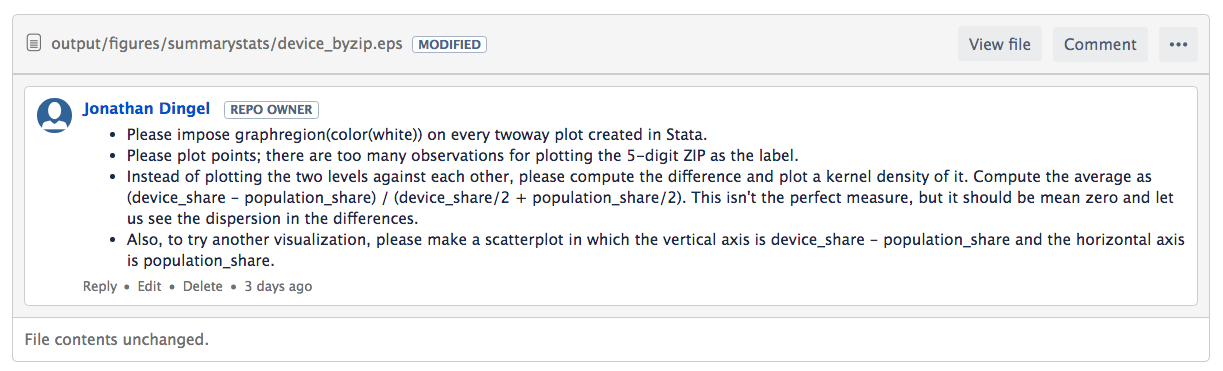
\includegraphics[width=.8\textwidth]{./figures/workflow/BitBucket_screenshot_commenting1.png}\end{center}
Ningyin can reply to comment to ask for clarification, and Jonathan can link to this commit comment when assigning tasks.

\subsubsection{Comment on a line}
You can also write comments on individual lines of a file.
Jonathan spotted a ``force'' option on line 99 of \texttt{code/gen\_census\_data.do} and wrote a comment seeking clarification.
He embeds his code suggestion as part of the comment, complete with BitBucket's language-specific syntax highlighting.
\begin{center}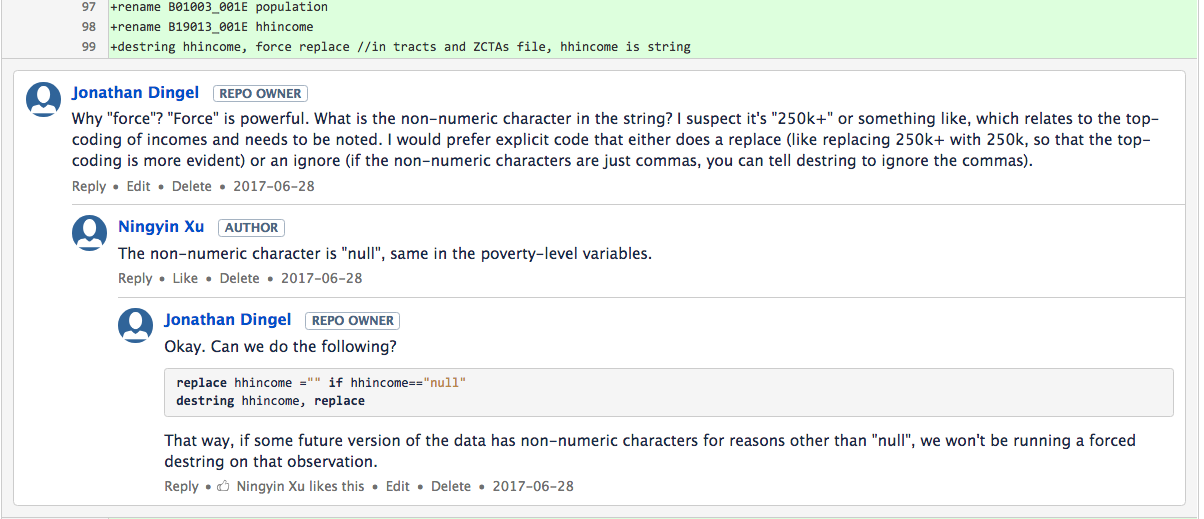
\includegraphics[width=\textwidth]{./figures/workflow/BitBucket_screenshot_commenting2.png}\end{center}

